\RequirePackage[l2tabu,orthodox]{nag}

% TODO: decide if one-sided/two-sided % Affects margins and stuff
%\documentclass[headsepline,footsepline,footinclude=false,fontsize=11pt,paper=a4,listof=totoc,bibliography=totoc,BCOR=12mm,DIV=12]{scrbook} % two-sided
\documentclass[headsepline,footsepline,footinclude=false,oneside,fontsize=11pt,paper=a4,listof=totoc,bibliography=totoc]{scrbook} % one-sided

% TODO: change citation style in settings
\PassOptionsToPackage{table,svgnames,dvipsnames}{xcolor}

\usepackage[utf8]{inputenc}
\usepackage[T1]{fontenc}
\usepackage[sc]{mathpazo}
\usepackage[ngerman,american]{babel}
\usepackage[autostyle]{csquotes}
\usepackage[%
  backend=biber,
  url=false,
  style=alphabetic,
  maxnames=4,
  minnames=3,
  maxbibnames=99,
  giveninits,
  uniquename=init]{biblatex} % TODO: adapt citation style
\usepackage{graphicx}
\usepackage{scrhack} % necessary for listings package
\usepackage{listings}
\usepackage{lstautogobble}
\usepackage{tikz}
\usepackage{pgfplots}
\usepackage{pgfplotstable}
\usepackage{booktabs}
\usepackage[final]{microtype}
\usepackage{caption}
\usepackage[hidelinks]{hyperref} % hidelinks removes colored boxes around references and links
% Mine
\usepackage{comment}
\usepackage[acronym,automake]{glossaries}

\makeglossaries

\newacronym{cdp}{CDP}{Collaborative Design Platform}
\newacronym{cve}{CVE}{Collaborative Virtual Environment}
\newacronym{vr}{VR}{Virtual Reality}
\newacronym{wa}{WA}{Workspace Awareness}
\newacronym{sa}{SA}{Situation Awareness}
\newacronym{vb}{VB}{Virtual Building}
\newacronym{tum}{TUM}{Technical University of Munich}
%\newacronym{la}{LA}{Los Angeles}
%\newacronym{us}{US}{United States}

%\bibliography{bibliography}

\setkomafont{disposition}{\normalfont\bfseries} % use serif font for headings
\linespread{1.05} % adjust line spread for mathpazo font

% Add table of contents to PDF bookmarks
\BeforeTOCHead[toc]{{\cleardoublepage\pdfbookmark[0]{\contentsname}{toc}}}

% Define TUM corporate design colors
% Taken from http://portal.mytum.de/corporatedesign/index_print/vorlagen/index_farben
\definecolor{TUMBlue}{HTML}{0065BD}
\definecolor{TUMSecondaryBlue}{HTML}{005293}
\definecolor{TUMSecondaryBlue2}{HTML}{003359}
\definecolor{TUMBlack}{HTML}{000000}
\definecolor{TUMWhite}{HTML}{FFFFFF}
\definecolor{TUMDarkGray}{HTML}{333333}
\definecolor{TUMGray}{HTML}{808080}
\definecolor{TUMLightGray}{HTML}{CCCCC6}
\definecolor{TUMAccentGray}{HTML}{DAD7CB}
\definecolor{TUMAccentOrange}{HTML}{E37222}
\definecolor{TUMAccentGreen}{HTML}{A2AD00}
\definecolor{TUMAccentLightBlue}{HTML}{98C6EA}
\definecolor{TUMAccentBlue}{HTML}{64A0C8}

% Settings for pgfplots
\pgfplotsset{compat=newest}
\pgfplotsset{
  % For available color names, see http://www.latextemplates.com/svgnames-colors
  cycle list={TUMBlue\\TUMAccentOrange\\TUMAccentGreen\\TUMSecondaryBlue2\\TUMDarkGray\\},
}

% Settings for lstlistings
\lstset{%
  basicstyle=\ttfamily,
  columns=fullflexible,
  autogobble,
  keywordstyle=\bfseries\color{TUMBlue},
  stringstyle=\color{TUMAccentGreen}
}

\addbibresource{zoteroExport.bib}
%\nocite{*} % print complete bibliography, even if not cited

% TODO: change thesis information
\newcommand*{\getUniversity}{Technische Universität München}
\newcommand*{\getFaculty}{Department of Architectural Informatics}
\newcommand*{\getTitle}{Workspace Awareness in Virtual Reality: Digital collaboration in architectural design}
\newcommand*{\getTitleGer}{Workspace Awareness in Virtueller Realität: Digitale Kollaboration im Kontext des Architektonischen Entwerfens}
\newcommand*{\getAuthor}{Vadym Strelchenko}
\newcommand*{\getDoctype}{Master's Thesis in Informatics}
\newcommand*{\getSupervisor}{Supervisor}
\newcommand*{\getAdvisor}{Advisor}
\newcommand*{\getSubmissionDate}{Submission date}
\newcommand*{\getSubmissionLocation}{Munich}



\begin{document}

% Set page numbering to avoid "destination with the same identifier has been already used" warning for cover page.
% (see https://en.wikibooks.org/wiki/LaTeX/Hyperlinks#Problems_with_Links_and_Pages).
\pagenumbering{alph}
\input{pages/cover}

\frontmatter{}

\begin{titlepage}
  \centering

  \IfFileExists{logos/tum.pdf}{%
    \includegraphics[height=20mm]{logos/tum.pdf}
  }{%
    \vspace*{20mm}
  }

  \vspace{5mm}
  {\huge\MakeUppercase{\getFaculty{}}}\\

  \vspace{5mm}
  {\large\MakeUppercase{\getUniversity{}}}\\

  \vspace{20mm}
  {\Large \getDoctype{}}

  \vspace{15mm}
  {\huge\bfseries \getTitle{}}

  \vspace{10mm}
  {\huge\bfseries \foreignlanguage{ngerman}{\getTitleGer{}}}

  \vspace{15mm}
  \begin{tabular}{l l}
    Author:          & \getAuthor{} \\
    Supervisor:      & \getSupervisor{} \\
    Advisor:         & \getAdvisor{} \\
    Advisor:		 & \getAdvisorr{} \\
    Submission Date: & \getSubmissionDate{} \\
  \end{tabular}

  \IfFileExists{logos/faculty.pdf}{%
    \vfill{}
    \includegraphics[height=20mm]{logos/faculty.pdf}
  }{}
\end{titlepage}

\thispagestyle{empty}
\vspace*{0.8\textheight}
\noindent
I confirm that this \MakeLowercase{\getDoctype{}} is my own work and I have documented all sources and material used.

\vspace{15mm}
\noindent
\getSubmissionLocation{}, \_\_\_\_\_\_\_\_\_\_\_ \hfill \getAuthor{} \_\_\_\_\_\_\_\_\_\_\_

\cleardoublepage{}

\addcontentsline{toc}{chapter}{Acknowledgments}
\thispagestyle{empty}

\vspace*{20mm}

\begin{center}
{\usekomafont{section} Acknowledgments}
\end{center}

\vspace{10mm}

%TODO: Acknowledgments
Otago guys

freesound.org guys

3d models' creators

\cleardoublepage{}

\chapter{\abstractname}

\gls{vr} technology can benefit architectural design by providing an immersive and intuitive medium for collaboration, review and evaluation of the developed concepts.
I developed two early prototypes which indicated that users can be startled by certain unexpected events in immersive \gls{vr} environments.
To ensure satisfaction with the collaboration experience, I conducted a study on \gls{wa} during architectural collaboration in immersive \gls{vr} environments.
This paper presents the utility of using audio awareness in improving \gls{wa}.
I observed an overall positive effect of audio feedback on informing the users about changes happening in a digital shared workspace. Additionally, stereo headphones proved to be sufficient for delivering the auditory cues, especially, when combined with visual support.
In conclusion, awareness is only one of the factors that has to be taken into account when considering collaboration in immersive \glspl{ve}, along with interactions and user presentation.
This thesis supports previous research on audio awareness and shows its utility in the explored setting.

\begin{comment}
However, this immersiveness in combination with the inherently limited perceptual information available in \glspl{ve} creates a bizarre situation, where on one hand, the visual information is very convincing, but on the other, the familiar perceptual feedbacks from the environment and our own actions are stripped away.
Starting with the question of how this situation affects the satisfaction with collaboration experience, I arrive at the concept of \gls{wa}. I build upon the design of a previous study on \gls{wa} from the field of \gls{cscw} and adapt it into a study of architectural collaboration in an immersive \gls{vr} environment. 
The results of the conducted experiments support previous research and show the high benefit of using additional audio feedback to support \gls{wa}.
\end{comment}


\microtypesetup{protrusion=false}
\tableofcontents{}
\microtypesetup{protrusion=true}

\mainmatter{}

% !TeX root = ../main.tex
% Add the above to each chapter to make compiling the PDF easier in some editors.

\chapter{Introduction}
\begin{comment}
Chapter plan:
-Context: introduce CDP, explain the need for the VR collaboration component
-Problem description: explain that virtual working environment provides only limited information from the workspace (citing works on Workspace Awareness). Example/Motivation: giant buildings moving at and through you

-Research question??

-Hypothesis: hypothesise that additional auditory cues promote workspace awareness in collaborative VR
-Thesis Overview: provide a high-level overview of the contents of this thesis (Chapter 1 is about.., Chapter 2 is about..)
\end{comment}

% Context
% About CDP Gerhard
\gls{cdp} is a multidisciplinary project at the Technical University of Munich developed by the Chair of Architectural Informatics from the Department of Architecture, the Chair of Augmented Reality from the Department of Informatics, and the Leibniz-Rechnenzentrum M{\"u}nchen.
%About \gls{vr} Sketching Component Sofia
At its core, \gls{cdp} is a multi-touch table \cite[p.~5]{lampe_cdp//vr-sketching_2017} that provides a lot of  functionality useful in urban planning and design (i.e. the ability to interactively add new buildings at a given site on the map, sketch on the \gls{vb}s, run solar envelope and wind simulations, etc.). One of the latest  development directions for the table is a \gls{vr} component, which aims to provide the existing 3D sketching capabilities in an immersive \gls{vr} environment. With the addition of the this component, comes a question of implementing a \gls{cve} to allow multiple people to use it simultaniously.


%Motivation
%Lead to \gls{cdp} \gls{vr} Collaboration component
 In this \gls{cve} users would have to interact with real-sized \gls{vb}s, which points out the initial concern and the motivation for this work. Imagine 2 users performing their separate tasks in the same \gls{cve}: while User 1 is occupied with sketching on the \gls{vb}s and going through the new ideas for an urban district, User 2 is busy with positioning the buildings in the environment to be more esthetically pleasing. The main question was - how would the moving buildings be perceived by a user that is ocuppied with their own task (for example, in case when a \gls{vb} moves through User 1), and how would this influence the quality of collaboration and the satisfaction with the experience in general.  
 

 %Problem description
 This brings up a problem of awareness different users have of each other in the system. \cite{gutwin_descriptive_2002} argues that "... workspace awareness is much harder to maintain in groupware workspaces than in face-to-face environments, and it is often difficult or impossible to determine who else is in the workspace, where they are working, and what they are doing". Authors point out that this is due to certain properties that any virtual workspace, and collaborative software (groupware) in particular have. This is mostly due to the fact that these systems provide only limited information about their current state to the user \cite[p.~414-415]{gutwin_descriptive_2002}. This comes as no surprise, because it would be virtually impossible and impractical to implement all the intricate details of the real world in software that tries to automate it. 
  

 %Hypothesis 
 To overcome these limitations, a user must be provided with the essential information about the environment. In this project, I explore what effect additional auditory cues have on the \gls{wa} of the collaborators. This work extends the \gls{wa} study presented in \cite{gutwin_chalk_2011} by putting ephasis on \gls{wa} in an immersive \gls{vr} environment.
 

% Overview
\paragraph{}
Chapter 2 \textit{Collaboration and Cooperation} offers a look at the history and theory behind the current state of groupware (collaborative software) systems, including Collaborative Virtual Environments (CVEs). In Chapter 3 \textit{Collaboration in Similar Projects} I will review related projects and how they try to achieve comfortable collaboration. At the end I choose an approach to quantify comfortable collaboration experience. Chapter 4 \textit{Awareness: Quantifying Comfortable Collaboration} provides a deeper look into the awareness approach to groupware design and testing. In Chapter 5 \textit{Sonification} I review sonification as a tool to provide monitoring capabilities and enhance workspace awareness. Different approaches to sonification are presented. Chapter 6: \textit{Workspace Awareness in Immersive Virtual Reality Environment} guides the reader through the preparatory and the final user studies, gives the detailed description of the experiments, the results, and the discussion thereof.

%---------------Reference commands and structires

% \chapter{Introduction}\label{chapter:introduction}
% \section{Motivation: Teamwork is important. Creative thinking implies generation of ideas, collaboration, and communication. Virtual Reality (VR) is a great enhancement for creative thinking tool-set in architecture.}
%\subsection{Solution validation/evaluation in HCI: methods, and principles.}
\begin{comment}
Methodology: approach to solving the problem; chosen HCI methodology for the final evaluation - no idea
a. Chosen HCI evaluation methodology
\end{comment}


\begin{comment}
See~\autoref{tab:sample}, \autoref{fig:sample-drawing}, \autoref{fig:sample-plot}, \autoref{fig:sample-listing}.
\begin{table}[htpb]
  \caption[Example table]{An example for a simple table.}\label{tab:sample}
  \centering
  \begin{tabular}{l l l l}
    \toprule
      A & B & C & D \\
    \midrule
      1 & 2 & 1 & 2 \\
      2 & 3 & 2 & 3 \\
    \bottomrule
  \end{tabular}
\end{table}

\begin{figure}[htpb]
  \centering
  % This should probably go into a file in figures/
  \begin{tikzpicture}[node distance=3cm]
    \node (R0) {$R_1$};
    \node (R1) [right of=R0] {$R_2$};
    \node (R2) [below of=R1] {$R_4$};
    \node (R3) [below of=R0] {$R_3$};
    \node (R4) [right of=R1] {$R_5$};

    \path[every node]
      (R0) edge (R1)
      (R0) edge (R3)
      (R3) edge (R2)
      (R2) edge (R1)
      (R1) edge (R4);
  \end{tikzpicture}
  \caption[Example drawing]{An example for a simple drawing.}\label{fig:sample-drawing}
\end{figure}

\begin{figure}[htpb]
  \centering

  \pgfplotstableset{col sep=&, row sep=\\}
  % This should probably go into a file in data/
  \pgfplotstableread{
    a & b    \\
    1 & 1000 \\
    2 & 1500 \\
    3 & 1600 \\
  }\exampleA
  \pgfplotstableread{
    a & b    \\
    1 & 1200 \\
    2 & 800 \\
    3 & 1400 \\
  }\exampleB
  % This should probably go into a file in figures/
  \begin{tikzpicture}
    \begin{axis}[
        ymin=0,
        legend style={legend pos=south east},
        grid,
        thick,
        ylabel=Y,
        xlabel=X
      ]
      \addplot table[x=a, y=b]{\exampleA};
      \addlegendentry{Example A};
      \addplot table[x=a, y=b]{\exampleB};
      \addlegendentry{Example B};
    \end{axis}
  \end{tikzpicture}
  \caption[Example plot]{An example for a simple plot.}\label{fig:sample-plot}
\end{figure}

\begin{figure}[htpb]
  \centering
  \begin{tabular}{c}
  \begin{lstlisting}[language=SQL]
    SELECT * FROM tbl WHERE tbl.str = "str"
  \end{lstlisting}
  \end{tabular}
  \caption[Example listing]{An example for a source code listing.}\label{fig:sample-listing}
\end{figure}
\end{comment}
% !TeX root = ../main.tex
% Add the above to each chapter to make compiling the PDF easier in some editors.

\chapter{Literature Review}
\section{Information Processing}
\subsection{Information processing loop}
%introduce information processing loop and its components (Perception, Cognition, ...)
%Cues: show examples of how different perceptual cues (including auditory) are registered and processed by humans
\subsection{Auditory Cues}
%introduce auditory icons and earcons, explain the difference, and show the "alarming" role the sound can have 

\section{Awareness} %guide the reader from "giant buildings moving at you" to workspace awareness
\subsection{Situation Awareness}
%introduce SA as an up-to-date understanding of the immediate surroundings
\subsection{Workspace Awareness}
%present WA as being a subfield of SA that is more focused on day-to-day/routine/non-critical work, as opposed to SA that is used in nuclear field, pilot cockpit awareness studies, etc.
\subsection{Related Work: Shared Chulkboard Application}
%review the study by Carl Gutwin et al. that I'm basing my final study on
% !TeX root = ../main.tex
% Add the above to each chapter to make compiling the PDF easier in some editors.

\chapter{Experiments}
\section{Pilot Studies}
\subsection{Sound Speed and Type}
\subsection{Spatial Judgement}
\section{Workspace Awareness in Immersive Virtual Reality}
% Goal of the study

\paragraph{Methods}

% Participants, Procedure, Task

% Apparatus: Unity, Resonance Audio, Marshall Major II Stereo headphones, Vive

% Study Factors and Conditions: what my factors are, conditions ?= independer variables' values

% Experimental Design
\cite{gutwin_chalk_2011}:
* Awareness presentation was rotated for each participant, so that each presentation was seen in the same position an equal number of times
* There were eight trials in each condition, meaning that there were 24 data points measured per user in each session
* Only one dependent measurement was collected - reaction speed in determining the position of a moving \gls{vb}.

%Gutwin vs our study%
% TODO: add a pic: Gutwin's (vertical) and our (horizontal) working (sound) plane

\begin{table}[]
  \caption{Study comparison}
  \label{table:study_comp}
  \begin{tabular}{|l|l|l|}
  \hline
                             & Gutwin                & This study           \\ \hline
  Primary (distraction) task & Same as the secondary & Contextually related \\ \hline
  Working (sound) plane      & ?Vertical             & Horizonatal          \\ \hline
  Sound type                 & Auditory icons        & Auditory icons       \\ \hline
  Object of analysis         & Workspace awareness   & Workspace Awareness  \\ \hline
  \end{tabular}
\end{table}


\paragraph{Study limitations}
% the fact that we only sample the level 1 SA/WA (we won't be going into sampling direction of translation guesses from the participants)

\paragraph{Results}
% !TeX root = ../main.tex
% Add the above to each chapter to make compiling the PDF easier in some editors.

\chapter{Awareness: Quantifying Productive Collaboration Experience}

This chapter is going to introduce \gls{wa}, as a tool for developing productive collaboration systems. We will first take a look at the \gls{sa}, as it comprises a large chunk of the foundation that \gls{wa} builds upon.

\section{Situation Awareness}
% This section serves as a pre-cursor to the Workspace Awareness section, and shows the base that WA is built upon.

%Situation awareness itself
\gls{sa} is usually used in attention-critical and hazardous tasks, where failure to react to the a change in a system might cause serious and even lethal consequences. SA served as one of the base notions, on which the concept of the workspace awareness was built.

\gls{sa} has seen great development through its application in the aviation field, and \cite{endsley_situation_1988} defines it as a combination of: perception of the elements in the certain volume around the user at the given time; comprehension of the meaning of these elements; and the ability to project their state into the nearest future.


* Write about the jet fighter simulator somewhere
o Human factors?
o Levels of awareness // <- I will classify my system according to this in the end

\paragraph{Measurement}
\cite[p.~791-792]{endsley_situation_1988} reviews different approaches to the measurement of \gls{sa} that help system designers answer the fundamental question: "Does system A promote better SA than system B?". In the author's opinion, all the approaches that were available up to that point suffer from their own individual limitations. For example, the subjective approach, where the subject is asked to rate his \gls{sa} from 1 to 10 suffers from 2 major drawbacks: first, the subject is not aware of "what is really going on in the environment", and secondly, the outcome of the task can influence the rating. Similarly, the psychological approach suffers from the incomplete human-computer interfaces to monitor what is going on with the pilot at this moment, and what they are thinking about. Finally, if the questionnaires are used, the fact that humans are not that good at recalling past mental events comes into play. Another set of problems arises, if an attempt is made to solve the issue with the questionnaire approach by querying pilots in real-time, such as the pilots can start to attend to the information they are questioned upon more thoroughly or they can be under a heavy load at the moment of questioning, which would obstruct their answer.

Nevertheless, \cite{endsley_situation_1988} finds the biggest limitation of the mentioned approaches was that they attempted to evaluate only a single design issue at the time. All this leads \cite{endsley_situation_1988} to introduce the \gls{sagat}. The idea here is that, first, the task goes though goal-directed analysis to determine the \gls{sa} requirements: the goal, subgoals, decisions required to actualize the given subgoal, and the knowledge required on all three levels of \gls{sa} (\ref{fig:sagoalorientedtaskanalysis}). 
\begin{figure}
	\centering
	
\includegraphics[width=0.7\linewidth]{figures/placeholders/SA_goal_oriented_task_analysis}
	\caption{Format of Goal-Directed Task Analysis (totaly spizgenoe name from: \cite{endsley_direct_nodate})}
	\label{fig:sagoalorientedtaskanalysis}
\end{figure}
This should yield an extensive list of questions, which assess SA information the \gls{sa} information of primary and secondary importance (for an example of the results of such analysis, see the Fig. \ref{fig:sagoalorientedtaskanalysisresultexample}).
\begin{figure}
	\centering
	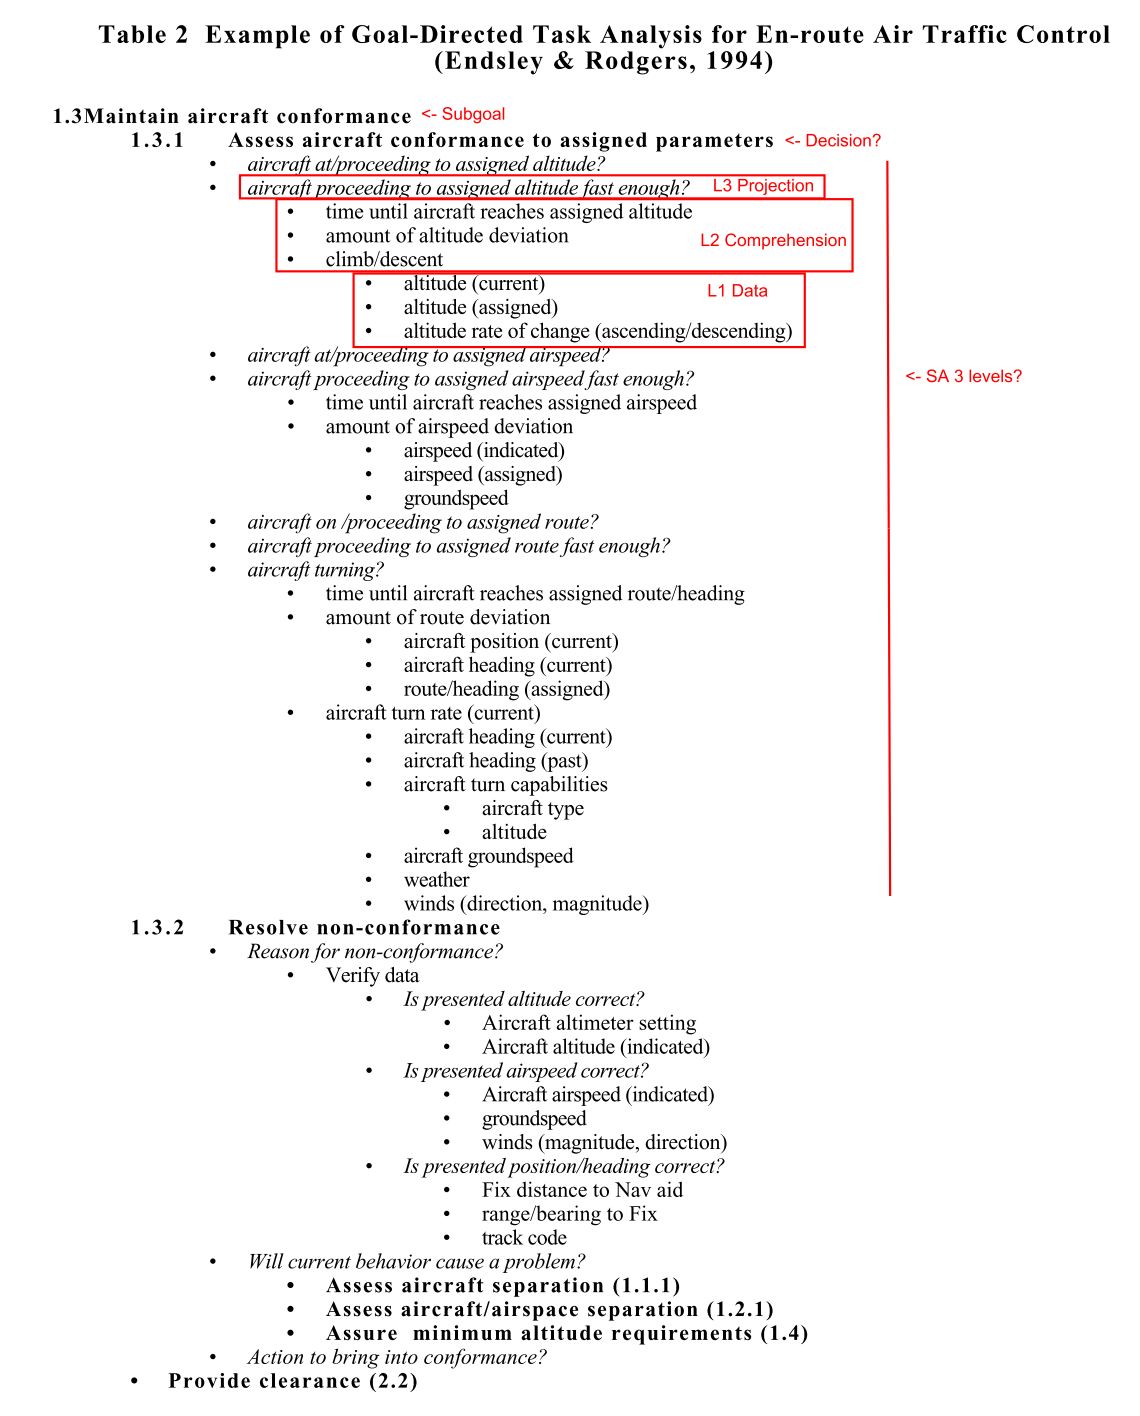
\includegraphics[width=0.7\linewidth]{figures/placeholders/SA_goal_oriented_task_analysis_result_example}
	\caption{Example of Goal-Directed Task Analysis for En-route Air Traffic Control (Endsley \& Rodgers, 1994) [from: \cite{endsley_direct_nodate}]}
	\label{fig:sagoalorientedtaskanalysisresultexample}
\end{figure}
Next, at some point in time, the simulation is halted, and the pilots are queried on the randomly selected questions from the list. When the simulation halts, all the control panels, the ?windshield of the jet-fighter, and other simulation elements are grayed-out. Not every pilot is queried on every question, the goal is to reach the desired statistical significance of the results by assessing a certain number of participants.

% This paragraph is a bit repetetive
By using this approach, it is possible to get a snapshot of the current situation in the point of view of the pilot, which is unbiased by the recall difficulties, and that can be compared to the actual situation after the experiment. Additionally, pilots' \gls{sa} is not artificially enhanced, because the questions do not always directly address the main goals in the current situation, but can concern secondary information, which is still relevant.

\cite{endsley_direct_nodate} notes that, since the introduction of \gls{sagat}, there is practical evidence that the method is valid, reliable, non-intrusive (in case of the halts are made at unpredictable time points), and is able to properly "reliably tap into memory stores" acting as a \gls{sa} index. 


o Bridge to Workspace Awareness


§ Workspace Awareness 
\gls{wa} is an extension of the idea of SA, and its adaptation to the day-to-day working scenarios. This is needed because, as authors put it: "sorting slides on a table does not seem very similar to air combat in a jet fighter", or in our case, to architectural collaboration in immersive VR environment.

o Relation to Situation awareness
o Relation to human factors’ research?
o Characteristics of awareness
* Measurement
SAGAT is sorta not applicable, because not so many elements to query upon.
o Bridge to Sonification: 
* Awareness - secondary/monitoring task \& sonification is great for monitoring -> use it for our experiment 


% !TeX root = ../main.tex
% Add the above to each chapter to make compiling the PDF easier in some editors.

\chapter{Summary}
% TODO: add more chapters here

\appendix{}

\microtypesetup{protrusion=false}
\listoffigures{}
\listoftables{}
\microtypesetup{protrusion=true}
\printbibliography
\printglossary[type=\acronymtype,title=Abbreviations]

\end{document}
